\section{Long-horizon static Occupancy World Models}

In this part, we introduce the W-DiT architecture and its corresponding optimization methods in Section \ref{sec:w-dit}, which form the foundation of our infinite-horizon static scene generation. In Section \ref{sec:fusion}, we briefly describe how to merge single-frame static scenes generated by W-DiT and infinitely extend them into closed-loop city-scale environments. Furthermore, in Section \ref{sec:agent}, we will demonstrate how to learn the possible distribution of agents layout from data and incorporate them into the scene to interact with test ego vehicle.

\subsection{Long-horizon stable generation with W-DiT}
\label{sec:w-dit}

\begin{figure}[tb]
    \centering
    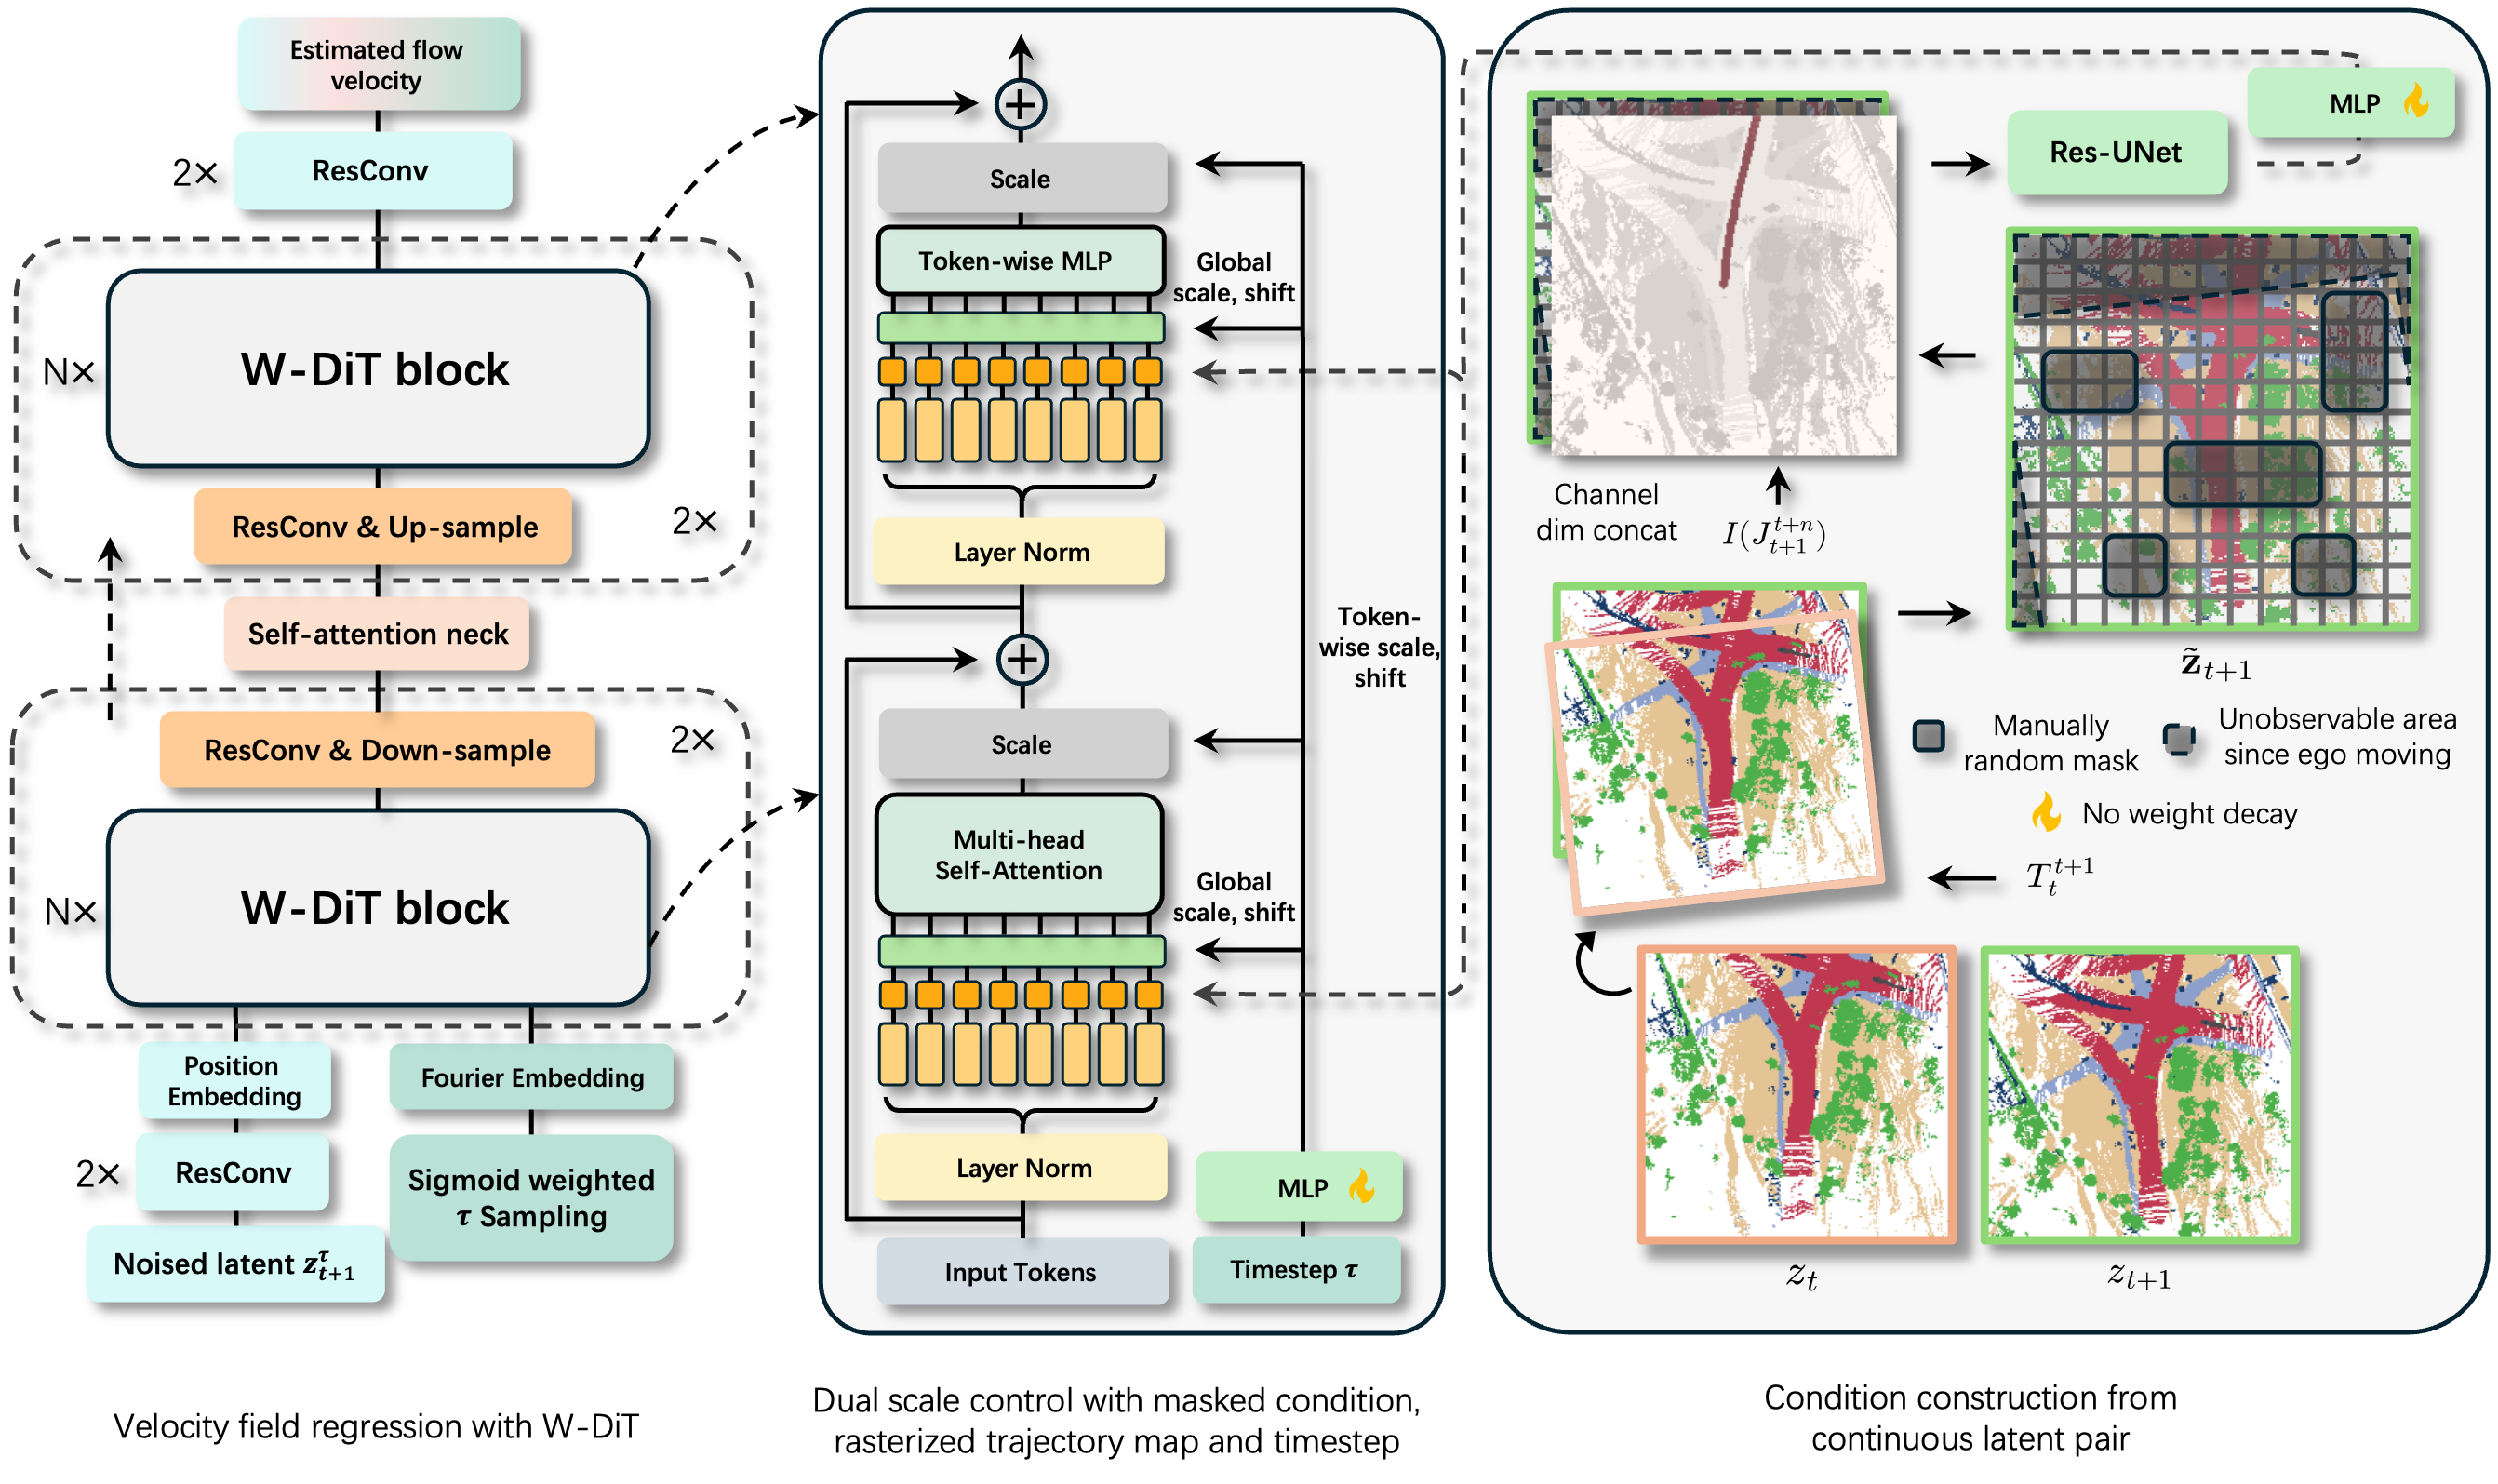
\includegraphics[width=\linewidth]{figures/W-DiT.png}
    \caption{Illustration of structure to generate road map of $t+1$ from condition at timestep t. Here, $t$ represents the sequence frame index, and $\tau$ denotes the probability flow timestep. Different from classic temporal concatenation in the input, the core insight of this paradigm design is to transform temporal generation into scene completion at a single time point. This token-wise scale and shift condition injection method allow us can precisely control spatial rigid transformation during long-horizon generation. $I(-)$ stand for rasterization process of given future trajectory $J_{t+1}^{t+n}$. The latent representations $z_t$ and $z_{t+1}$ ($\in \mathbb{R}^{H \times W \times C_z}$) at bottom right corner are visualized as decoded BEV occupancy maps for intuitive illustration.}
    \label{fig:W-DiT}
\end{figure}

A fundamental distinction between occupancy sequences and RGB sequences is that perspective shifts of occupancy sequences can be represented with rigid transformations. Despite this advantage, most existing occupancy world models na\"ively inherit the 2+1D information aggregation approach from video generation. We found that a geometry-aware alternative yields substantial improvements in long-term stability, perspective controllability, and spatial consistency.

Formally, using an occupancy VAE  \cite{liu2025towards} (consisting of spatial compressor $\mathcal{E}$ and decoder $\mathcal{D}$), we can map the occupancy frames $\mathcal{O}_t, \mathcal{O}_{t+1}$ to their respective latent representations $\mathbf{z}_t, \mathbf{z}_{t+1} \in \mathbb{R}^{H \times W \times C_z}$, where $t$ denotes time index. Our aim is to model the joint predictive distribution over an extended future horizon: given an initial latent state $\mathbf{z}_0$ and a sequence of future ego-trajectories $J_{0:K+\sigma}$, our goal is to auto-regressively estimate:
\vspace{-2mm}
\begin{equation}
    P(\mathbf{z}_{1:K} | \mathbf{z}_0, J_{0:K+\sigma}) = \prod_{i=1}^{K} P_{\theta}(\mathbf{z}_{i} | \mathbf{z}_{i-1}, J_{i-1:i+\sigma-1}),
\end{equation}%
where K is the overall forecast horizon and $K + \sigma$ stand for the length of trajectory. When $K \geq 10^{3}$, standard autoregressive formulations inevitably suffer from severe compounding errors, leading to structural drift and spatial inconsistency over time. To enforce ultra-long-term stability and fidelity, we propose the W-DiT (Warp-DiT) block (Figure \ref{fig:W-DiT}). Unlike conventional RGB-based world models, which require the network to implicitly hallucinate perspective changes, the core design of W-DiT lies in explicitly utilizing a sequence of deterministic rigid transformation matrices—derived from the trajectory $J$—to warp the spatial latent representations, thereby bounding geometric accumulation error.
 

Specifically, to have the rigid transformation matrices, we assume a planar motion on the $XY$-plane, we constrain the vertical velocity and roll/pitch rotations to zero. Therefore, we can define $\mathbf{T}_{t}^{t+1} = \exp(\widehat{\xi}_t \Delta t)$, where $\exp(\cdot)$ denotes the matrix exponential, $\xi_t = \mathcal{M}(\boldsymbol{a}_t)$ is the twist vector corresponding to $\boldsymbol{a}_t = [v_{x,t}, v_{y,t}, \omega_t]^\top$, the hat operator $\widehat{\cdot}$ converts the twist $\xi_t = [v_{x,t}, v_{y,t}, 0, 0, 0, \omega_t]^\top$ into its matrix form $\widehat{\xi}_t = [ [\boldsymbol{\omega}]_\times, \mathbf{v}; 0 ] \in \mathbb{R}^{4\times4}$, with the planar velocity vector $\mathbf{v} = [v_{x,t}, v_{y,t}, 0]^\top$ and yaw rate vector $\boldsymbol{\omega} = [0, 0, \omega_t]^\top$. Here, $[\cdot]_\times$ denotes the skew-symmetric matrix operator.

Subsequently, by applying the rigid transformation $\mathbf{T}_{t}^{t+1}$, we forward-warp $\mathbf{z}_t$ to the viewpoint at $t+1$ to obtain the warped latent $\hat{\mathbf{z}}_{t+1}$. Due to the ego-vehicle's motion, certain spatial regions in this warped latent inevitably fall outside the sensor's field of view or become occluded. To explicitly account for this, we can deterministically compute a binary visibility mask $\mathbf{M}_{\text{vis}} \in \{0, 1\}^{H \times W}$ derived purely from the known geometry, where observable regions are set to 1 and unobservable ones to 0. However, since the physical displacement between adjacent frames is relatively small (e.g., 3 to 4 meters given $\Delta t = 0.5\text{s}$), relying solely on $\mathbf{M}_{\text{vis}}$ is insufficient and encourages the model to degenerate into a trivial shortcut of directly copying the inputs, which severely hinders robust representation learning. Therefore, following MAE \cite{he2022masked}, we introduce an additional random mask $\mathbf{M}_{\text{rand}} \in \{0, 1\}^{H \times W}$, whose elements are sampled from a Bernoulli distribution $\mathcal{B}(1 - p)$, with $p$ being the given masking ratio. The final conditioned latent $\tilde{\mathbf{z}}_{t+1}$ is then formulated as $\tilde{\mathbf{z}}_{t+1} = (\mathbf{M}_{\text{vis}} \odot \mathbf{M}_{\text{rand}}) \odot \hat{\mathbf{z}}_{t+1}$, where $\odot$ denotes the Hadamard product, and the spatial masks are broadcast across the channel dimension $C_z$. 

Next, instead of fusing the future action with $\tau$ directly \cite{gu2024dome, shi2025come}, we rasterized these action to waypoints which align with time index $t+1$. Specifically, we represent the sequence of future actions as a set of physical waypoints $\mathcal{P}_t = \{\mathbf{p}_{t+i} \in \mathbb{R}^2 \}_{i=1}^\sigma$ projected onto the BEV plane. These waypoints are anchored in the ego coordinate system at time $t+1$, derived by cumulatively applying the previously defined rigid transformation matrices $\mathbf{T}_{t+1}^{t+\sigma}$. By sequentially connecting these waypoints, we construct a continuous geometric polyline that explicitly traces the intended path from the current ego position towards the future road surface and then rasterize it to $l_{t+1} \in \{0, 1\}^{H, W, 1} $. Here we use function $I(-)$ to represent this projection and rasterization process. Considering the interpolation error caused by the warping operation, we use a U-Net to refine the feature formed by concatenation of $l_{t+1}$ and $\tilde{\mathbf{z}}_{t+1}$, before injecting them to the backbone. Here, we use $f^{\prime}_{t+1} \in \mathbb{R}^{B,N,C_w}$ to represent token from condition at time t and trajectory, where $N = H \times W$.

After obtaining these features $\hat{f}_{t+1}$ aligned to time index $t+1$, we perform feature injection by applying token-wise scaling and shifting. Specifically, for global scale, shift, and gate regression, we still follow the same setting in original DiT, use timestep $\tau$ as input. Simultaneously, we employ a token-wise projection layer to regress the spatial control signal from $\hat{f}_{t+1}$:

\begin{equation*}
    [\gamma_{\text{global}}, \beta_{\text{global}}, \alpha_{\text{global}}] = \text{MLP}_{\text{time}}(\tau),  [\mathbf{\Gamma_{\text{token}}}, \mathbf{B}_{\text{token}}, \mathbf{A}_{\text{token}}] = \text{MLP}_{\text{cond}}(\hat{f}_{t+1})
\label{eq:dual_adaln_params}
\end{equation*}

From the main stream side, we obtain $z_{t+1}^{\tau}$ via a linear interpolation with the sampled gaussian noise $\epsilon$: $z_{t+1}^{\tau} = (1-\tau)\epsilon + \tau z_{t+1}$ and use $f_{t+1} \in \mathbb{R}^{B \times N \times C_w}$ to represent the tokenized feature feeded to W-DiT block. For the $i$-th token in the sequence, the modulation parameters are obtained via:

\begin{equation*}
\gamma^{(i)} = \gamma_{\text{global}} + \mathbf{\Gamma_{\text{token}}}^{(i)}, \quad \beta^{(i)} = \beta_{\text{global}} + \mathbf{B}_{\text{token}}^{(i)}, \quad \alpha^{(i)} = \alpha_{\text{global}} + \mathbf{A}_{\text{token}}^{(i)} 
\end{equation*}

With these dual-conditioned designs, the forward pass of the Multi-Head Self-Attention (MHSA) module in our W-DiT block is formulated as: $f_{t+1}^{\prime} = f_{t+1} + \boldsymbol{\alpha}_1 \odot \text{MHSA} \big( \boldsymbol{\gamma}_1 \odot \text{LN}(\mathbf{h}) + \boldsymbol{\beta}_1 \big)$, where $\boldsymbol{\gamma}_1 = [\gamma^{(1)}, \gamma^{(2)}, \dots, \gamma^{(N)}]^{\top} \in \mathbb{R}^{N \times C_w}$ denotes the stacked sequence of token-wise scale parameters, with $\boldsymbol{\beta}_1$ and $\boldsymbol{\alpha}_1$ defined analogously. We adopt the identical setting for $(\boldsymbol{\gamma}_2, \boldsymbol{\beta}_2, \boldsymbol{\alpha}_2)$ in subsequent MLP layer. Finally, after processing through all W-DiT blocks, the network outputs a prediction of the instantaneous velocity field at the probability flow timestep $\tau$. Let $v_\theta(z_{t+1}^{\tau}, \tau, \mathbf{c})$ denote our W-DiT network parameterized by $\theta$, where $\mathbf{c}$ compactly represents all the conditions we mentioned.

Following the recent success of flow models in achieving high-quality generation with fewer sampling steps \cite{liu2025towards, song2025hume, zhang2025epona}, we also optimize W-DiT by adopting a velocity loss objective. However, original MSE loss in flow matching provides a theoretically sound objective, our empirical investigations reveal that optimizing solely with it in the continuous latent space severely impedes model convergence. This phenomenon is a notorious challenge in continuous VAE-based generative models, where the MSE objective often forces the network into a ``mean trap''. To overcome this bottleneck, we propose a novel SNR-scaled Perception Loss. Our core insight is to leverage the inherently discrete and semantic nature of 3D occupancy. Rather than constraining the loss entirely within the continuous latent manifold, we explicitly project the denoised predictions back into the discrete occupancy space for direct supervision. Our overall objective function is:

\begin{equation}
 \mathcal{L}_{\mathrm{total}}(\theta) = \mathbb{E}_{\tau, \epsilon, z_{t+1}, \mathbf{c}} \bigg[ \left\| v_\theta - (z_{t+1} - \epsilon) \right\|_2^2 + \lambda \tau^2\frac{\mathbf{M}_{\mathrm{mask}}}{|\mathbf{M}_{\mathrm{mask}}|}\mathrm{CE}\bigg(\mathcal{O}_{t+1}, \mathcal{D}(z_{t+1}^{\tau} + (1-\tau)v_\theta)\bigg) \bigg]
\label{eq:total_loss}
\end{equation}

where $\mathbf{M}_{\mathrm{mask}} = \mathbf{M}_{\text{vis}} \odot \mathbf{M}_{\text{rand}}$ and $\lambda$ were used to balance different components. In the second term, at flow timestep $\tau$, we first recover the denoised latent representation $\hat{z}_{t+1}=z_{t+1}^{\tau} + (1-\tau)v_\theta(z_{t+1}^{\tau}, \tau, \mathbf{c})$ using the current velocity field presented by $v_\theta$ without any sampling. Then we feed $\hat{z}_{t+1}$ into the frozen VAE decoder $\mathcal{D}$ to reconstruct the occupancy logits $\hat{\mathcal{O}}_{t+1} = \mathcal{D}(\hat{z}_{t+1})$ for mask-region only Cross-Entropy (CE) loss between $\hat{\mathcal{O}}_{t+1}$ and $\mathcal{O}_{t+1}$.

Crucially, we introduce a time-dependent scaling factor $\tau^2$ to this perception loss, which we ablate in Sec. \ref{sec:ablation}. This term guarantees that, when $\tau$ is large (indicating a low-noise regime closer to the target data), the weight exponentially increases. This encourages the network to refine fine-grained geometric boundaries and semantic details. 

\subsection{Multi-kilometer road map fusion from single frames}
\label{sec:fusion}

As detailed in Sec. \ref{sec:w-dit}, our W-DiT is capable of stably rolling out thousands of static map frames. While the stochastic nature of flow models effectively bypasses the data scarcity bottleneck of traditional HD maps, the generated outputs remain discrete, ego-centric local scenes. Furthermore, naive fusion strategies, such as temporal averaging, tend to aggressively over-smooth crucial high-frequency details during sequence aggregation, because of the temporal inconsistency in the forecasted frames.

Our strategy consists of two components: key-frame based fusion and branch road detection: We first propose a two-pass keyframe-based fusion heuristic (detailed in Alg.~\ref{alg:keyframe_fusion} in Appendix~\ref{sec:appendix_algorithms}). Given local occupancy predictions and their global poses, we first aggregate a minimally overlapping keyframe subset to establish a sharp foundational map $\mathcal{M}_{\text{global}}$. Subsequently, after a gravity alignment step, the redundant non-keyframes are used to robustly inpaint spatial gaps via threshold-based voting and morphological cleaning.

To enable unbounded map expansion, we systematically identify valid extensible frontiers within $\mathcal{M}_{\text{global}}$. By applying morphological skeletonization to the road manifold, we extract a topological graph to isolate candidate branch points (Alg.~\ref{alg:branch_detection} in Appendix~\ref{sec:appendix_algorithms}). A Dual-Probing Filtering mechanism—comprising topological and 3D semantic probes—is then employed to reject collision-prone directions. By selecting two valid disjoint endpoints and connecting them via a collision-free spline, we prompt W-DiT to autoregressively synthesize the missing intermediate occupancy. This autoregressive bridging paradigm elegantly closes the loop, enabling the unbounded, procedural generation of diverse autonomous driving scenarios from a single prompt occupancy.

\begin{figure}[tb]
    \centering
    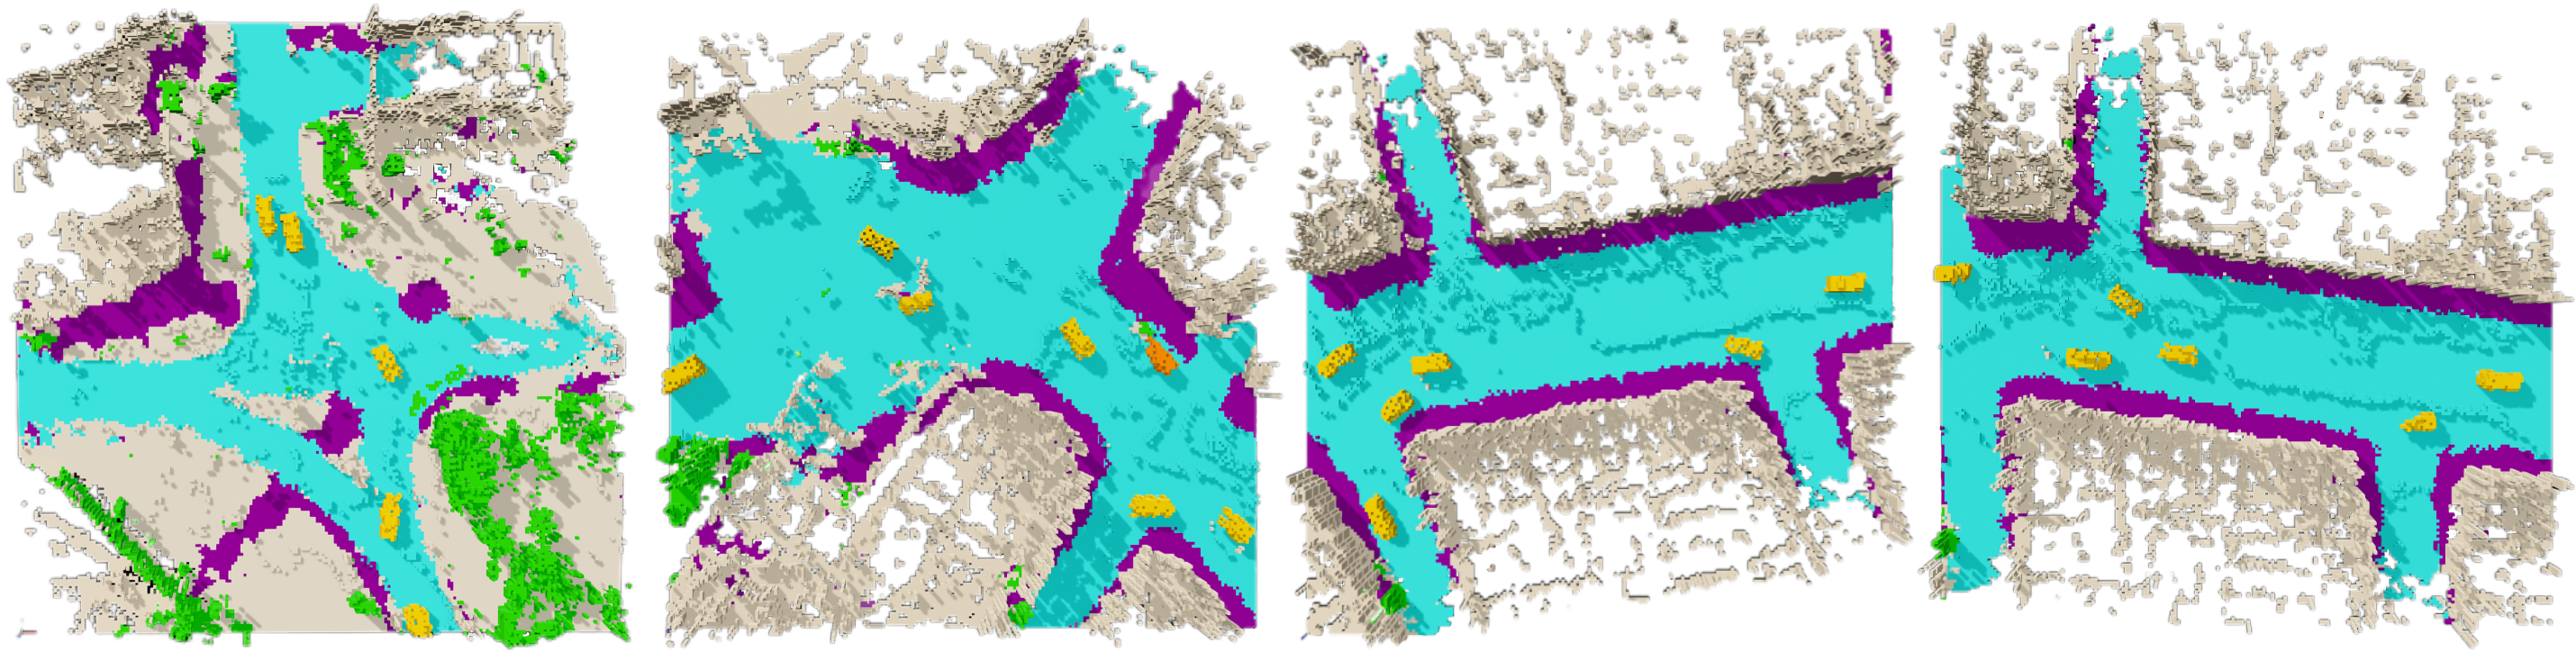
\includegraphics[width=\linewidth]{figures/with_agents_final.png}
    \caption{\textbf{Agent initialization within generated static maps.} Each panel displays a 200x200 voxel crop centered on the (unrendered) ego-vehicle from $\mathcal{M}_{\text{global}}$. The first two panels show distinct generated scenes, the third and fourth panels demonstrate the model's multimodality: two different plausible layouts generated for the same revisited location. Orange vehicles (second panel) are stationary.}
    \label{fig:with_agent}
\end{figure}

\subsection{Agent generation and control with static road map}
\label{sec:agent}

Having constructed the city-scale static map $\mathcal{M}_{\text{global}}$ (with explicit lane graphs extracted via Alg. 3), we next populate the environment with plausible initial agent states. Unlike log-replay methods, our procedurally generated topologies are generated, necessitating a generative approach for traffic layouts.

Formally, our objective is to model the conditional probability distribution of the agent layout given 1 frame of static environment: $P(\mathcal{A} | \mathbf{z}_{t})$, where $\mathcal{A} = \{(x_i, y_i, s_i)\}_{i=1}^N$ denotes the set of vehicle centers $(x_i, y_i)$ motion states $s_i \in \{\text{dynamic}, \text{static}\}$ and $\mathbf{z}_{\text{static}}$ is cropped from a previously fused large map given a random pose. To make this distribution tractable for our flow-based generative framework, we map the discrete set $\mathcal{A}$ into a continuous 2D spatial heatmap $\mathcal{H}$, encoding static and dynamic vehicles as positive and negative standard Gaussian kernels, respectively. Then we train a compact Diffusion Transformer (DiT-S) to learn the continuous distribution $P(\mathcal{H} | \mathbf{z}_{t})$. To prevent the DiT-S from overfitting and memorizing small-scale dataset layouts, we apply multiple spatial augmentations during training (detailed in Appendix)

During inference, the sampled heatmap $\mathcal{H}$ is discretized via Non-Maximum Suppression (NMS) to extract individual vehicle instances. Each vehicle is then projected onto the nearest lane to establish a kinematically feasible initial yaw. In figure \ref{fig:with_agent}, we visualize several samples after add the agents to their initial pose. Finally, we employ A* routing and the extended 2D Intelligent Driver Model (2D-IDM) \cite{kesting2010enhanced} to roll out microscopic kinematic trajectories toward randomly selected junctions in $\mathcal{M}_{\text{global}}$ (Alg.~\ref{alg:idm_rollout} in Appendix~\ref{sec:appendix_algorithms}). While we utilize classic heuristics to validate simulation feasibility, our  initialized map topology and agent poses guarantee plug-and-play compatibility with any modern learning-based trajectory forecasting model.

